\documentclass[12pt, a4paper]{report}
\usepackage{a4wide}
\usepackage{anysize}
\usepackage[centertags]{amsmath}
\usepackage{amsfonts,amssymb,amsthm}
\usepackage{graphicx}
\usepackage{natbib}
\usepackage{wrapfig}
\usepackage{iitbieortitle}
\usepackage{pgf}
\usepackage{subcaption}

%\usepackage{fullpage}
%\usepackage{rotating}
\usepackage{printlen}
\usepackage[ruled,vlined]{algorithm2e}
\usepackage{amsmath}
\usepackage{tikz}           % Package for 
\usepackage{algorithm}
\usepackage{subcaption}
\renewcommand{\baselinestretch}{1.2} %line spacing
\marginsize{1.2in}{1.2in}{1in}{1in}   %left right top bottom
\textwidth 6in
% Title Page

\begin{document}



\pagenumbering{roman}
\pagestyle{plain}
\def\title{Microstructure Statistics}
\def\what{Dual Degree Project}
\def\who{Iyer Adithya Jairam (16D110011)}
\def\guide{Prof. M P Gururajan and Prof. Hina Gokhale}

\titlpage
\tableofcontents
\listoffigures


\newpage
\pagenumbering{arabic}



\chapter{Data Description and Pre-processing}

\section{Data Description}
The data generated was in the form of .dat files, with each .dat file representing one microstructural image. Each image consisted of $2048* 2048$ pixels, with each pixel representing the composition at the point, ie. the pixel values ranged between 0 and 1. The pixels with values $>=0.5$ are considered as precipitates in our analysis.

The generated microstructure for $200000$ time steps was usually sampled after every $100$ time steps, thus the total number of images obtained were $2000$. For some cases, sampling after every 200 time steps produced 1000 images. Thus, all analysis was done on $2000$/$1000$ images each image having a resolution of $2048*2048$. Three sets each of Cahn-Hilliard circular microstructures and hexagonal microstructures were generated, with the compositions for the minor component set at $0.3$, $0.4$ and $0.5$ for each respectively.


\section{Data Pre-processing}
Statistical analysis of shape, size and distribution often requires the image pixel values to be more differential for gradient calculations, and binary for image shape and size quantification. Thus these data pre-processing steps are essential to improve precision of the algorithms henceforth mentioned.

The images are first made continuous by convolution of the image with a $5*5$ Gaussian filter to remove shape discontinuities, and make the gradient($1st$ derivative) smooth. After smoothening, the microstructure was binarized by replacing pixel values $>=0.5$ by 1 and $<0.5$ by 0. This binary microstructure is henceforth used as the image for study.

\begin{figure}[H]
\centering
\begin{subfigure}{0.45\textwidth}
  \centering
  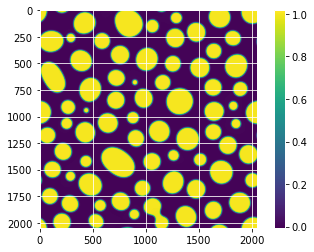
\includegraphics[width=0.9\textwidth]{Pictures/DataProcessingNonSmoothened.png}
  \caption{Raw microstructure Image}
  \label{img:microstrImg}
\end{subfigure}
\begin{subfigure}{.45\textwidth}
  \centering
  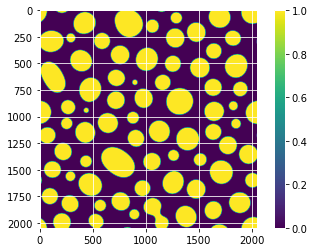
\includegraphics[width=0.9\textwidth]{Pictures/DataProcessingSmoothened.png}
  \caption{Smoothened and binarized image}
  \label{img:MicrostrImg}
\end{subfigure}
\caption{Visualizing data}
\label{fig:test}
\end{figure}

%%%%%%%%%%%%%%%%%%%%%%%%%%%%%%%%%%%%%%%%%%

\chapter{2 Point Statistics}
\section{Formulation}
Quantifying the spatial distribution of states in a microstructure can help us quantify the density of precipitate and define how isotropic or anisotropic a particular microstructure is. We calculate these distributions in terms of the microstructure probability function $m_s^n$, defined as the probability of finding the local state $n$ at the spatial location $s$. In our binary microstructures, the $m_s^n$ values are either $1$ or $0$, ie. a local state is either present or not present at a particular spatial location. 

We extend this formulation to include 2 local states, and define $f_t^{n_1n_2}$ as the probability of finding local state $n_1$ at a spatial location while simultaneously finding $n_2$ at a spatial location $t$ vector away from the original spatial location. This value can be calculated as follows:

$f_t^{n_1n_2} = \frac{1}{S}\sum_{s=0}^{S-1} {m_s^{n_1}}{m_{s+t}^{n_2}}$

We solve the above sum by taking the $LHS$ and the $RHS$ into the Fourier space and apply the Convolution theorem to the $RHS$ expression. This gives us the Fourier transform of $f_t^{n_1n_2}$ as:


$$
F_k^{n_1n_2} = \sum_{s=0}^{S-1}{m_s^{n_1}}{m_{s+t}^{n_2}} = \frac{1}{S} \sum_{s=0}^{S-1}{m_s^{n_1}}{e^{\frac{-2{\pi}isk}{S}}}  \sum_{z=0}^{S-1}{m_z^{n_2}}{e^{\frac{2{\pi}izk}{S}}}
$$

We then take the inverse Fourier transform of the above expression to calculate the 2 point correlations. 

Here, if $n_1$ and $n_2$ are the same local state in our binary microstructures({1,1} or {0,0}), the $f_t^{n_1n_2}$ values would represent the \textbf{auto-correlations} of the local states 1 and 0 respectively. Alternatively, if $n_1$ and $n_2$ are the different local states, ie. ({1,0} or {0,1}), the $f_t^{n_1n_2}$ values would correspond to the cross-correlation of the 2 local states.

\section{Algorithm}
We utilize the python library $numpy$ to calculate the auto-correlation and cross-correlation values, since it supports swift calculation of Fourier and inverse-Fourier transform. The microstructure probability function $m_s^{n_i}$ is calculated for each of the $i^{th}$ local state, and stored as $numpy$ arrays mi(m1, m2 etc.). The flowchart below summarizes the process followed in calculating the correlations.

\usetikzlibrary{shapes.geometric, arrows}
\tikzstyle{process} = [rectangle, minimum width=3cm, minimum height=1cm, text centered, draw=black]
\tikzstyle{arrow} = [thick,->,>=stealth]
\begin{center}
\begin{tikzpicture}[node distance=2cm]
\node (start) [process] {Calculate m1 and m2};
\node (in1) [process, below of=start] {Fourier transform of m1 and m2(M1 and M2) };
\node (in2) [process, below of=in1] {Inverse Fourier Transform of M1*conjugate(M2)/(No of pixels)};
\node (in3) [process, below of=in2] {Absolute value, followed by reshaping(fftshift) to image size};
\draw [arrow] (start) -- (in1);
\draw [arrow] (in1) -- (in2);
\draw [arrow] (in2) -- (in3);
\end{tikzpicture}
\end{center}

\section{Visualization}
The probability correlation values are visualized by representing the probability values as colors of varying intensities, centred at the origin of the image. Once the correlations are captured, we can calculate the radial probability distribution, as well as the probability distributions at various angular sectors. These visualizations are presented below:

\begin{figure}[H]
\centering
\begin{subfigure}{.45\textwidth}
  \centering
  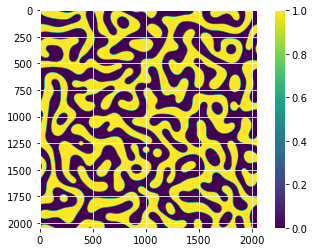
\includegraphics[width=0.9\textwidth]{Pictures/2 Point/2_point_binary_image.jpeg}
  \caption{Raw microstructure Image}
  \label{img:microstrImg}
\end{subfigure}
\begin{subfigure}{.45\textwidth}
  \centering
  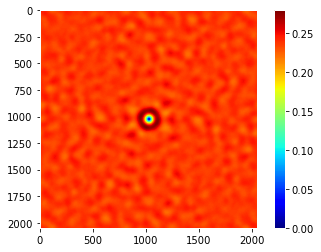
\includegraphics[width=0.9\textwidth]{Pictures/2 Point/2_point_stats_bw.jpeg}
  \caption{Cross Correlation}
  \label{img:microstrImg}
\end{subfigure}
\begin{subfigure}{.45\textwidth}
  \centering
  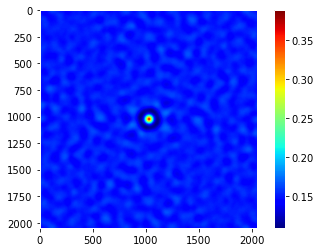
\includegraphics[width=0.9\textwidth]{Pictures/2 Point/2_point_stats_ww.jpeg}
  \caption{1-1 Auto-Correlation}
  \label{img:microstrImg}
\end{subfigure}
\begin{subfigure}{.45\textwidth}
  \centering
  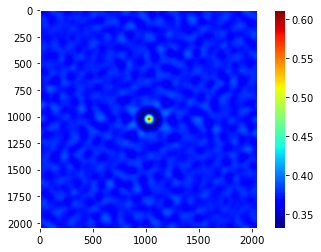
\includegraphics[width=0.9\textwidth]{Pictures/2 Point/2_point_stats_bb.jpeg}
  \caption{0-0 Auto-Correlation}
  \label{img:microstrImg}
\end{subfigure}
\begin{subfigure}{.45\textwidth}
  \centering
  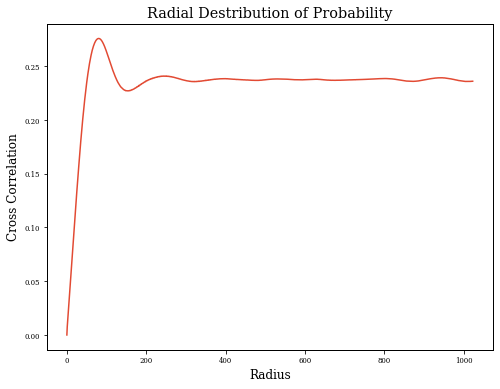
\includegraphics[width=0.9\textwidth]{Pictures/2 Point/2_point_stats_radial.jpeg}
  \caption{Radial Cross Correlation}
  \label{img:microstrImg}

\end{subfigure}

\caption{Visualizing Correlations}
\label{fig:test}
\end{figure}

%%%%%%%%%%%%%%%%%%%%%%%%%%%%%%%%%%%%%%%%%%%%%%

\chapter{Level Set Methods and Velocity Formulation}

Calculating velocity of interface is important since it gives us a good metric to judge pace of precipitate growth, and understand the inherent qualitative properties of the 2 phases. We have used the Level Set Method to quantify the orthogonal velocity at the interface of the 2 phases.
 
\section{Level Set Methods: Formulation}
The problem statement can broadly be broken down into 3 parts, locating the interface, finding the normal to the interface to suggest direction of movement and finding the magnitude of the interface velocity. We study the 3 parts separately:

\subsection{Contouring or Interface Location}
We define the interface pixels as the pixels which have at least one bordering(vertical, horizontal and diagonal) precipitate pixel. Thus for a single pixel precipitate, we would have 8 bordering interface pixels. The presence of diagonally neighbouring points do not harm our calculations, since we smoothen the binary image, and the gradients formed post smoothening are nearly equal in orthogonal and diagonal neighbours. The figure below illustrates the contours found for a hexagonal microstructure. Because the contours are really fine, the picture will have to be zoomed in to notice the contours as computer rendering makes the faint lines more transperent.

\begin{figure}[H]
\centering
\begin{subfigure}{.6\textwidth}
  \centering
  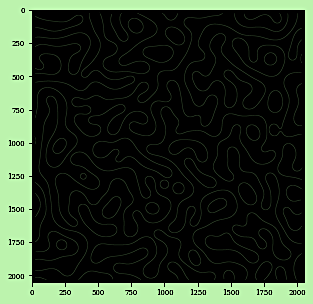
\includegraphics[width=0.9\textwidth]{Pictures/Level Set/level_set_contours.png}
  \caption{Contours on the microstructure}
  \label{img:microstrImg}
\end{subfigure}
\label{fig:test}
\end{figure}

\subsection{Interface direction}
The interfacial velocity and direction of a growing or shrinking precipitate can be captured by applying level set methods. This involves first converting the binary image into a continuous \textbf{signed difference function}($\Phi$). We do this by first smoothening the image by convolving a 5x5 gaussian kernel across the whole image, and then subtracting 0.5 to make the interface pixels close to 0.  

Once we have obtained the Signed Difference Function($\Phi$), we can apply Level Set Algorithms to find the interface normal vector and the velocity. The normal vector $\vec{N}$ and the velocity magnitude $|\vec{V}|$.

$\vec{N} = -\frac{\nabla\Phi}{|\nabla\Phi|}$

$|\vec{V}| = \frac{\frac{d\Phi}{dt}}{|\nabla\Phi|}$

Here, the sign of $\frac{d\Phi}{dt}$ decides whether an interface is expanding or contracting. Furthermore, $\frac{d\Phi}{dt}$ was calculated by interpolating a line through 4 points, to make the derivatives more representative of the actual curve.

\section{Algorithm}

We followed the following process while calculating the interface velocities of the precipitates in our microstructures. 

\usetikzlibrary{shapes.geometric, arrows}

\tikzstyle{process} = [rectangle, minimum width=3cm, minimum height=1cm, text centered, draw=black]
\tikzstyle{arrow} = [thick,->,>=stealth]
\begin{center}
\begin{tikzpicture}[node distance=2cm]
\node (start) [process] {Find interface pixels};
\node (in1) [process, below of=start] {Calculate Signed Difference Function $\Phi$};
\node (in2) [process, below of=in1] {Calculate interface normal vector($\vec{N}$) and velocity magnitude($|\vec{V}|$)};
\node (in3) [process, below of=in2] {Multiply $\vec{N}$ and $|\vec{V}|$ to get velocity vector};
\node (in4) [process, below of=in3] {Plot quiver plot of velocity vectors by selectively selecting points};
\draw [arrow] (start) -- (in1);
\draw [arrow] (in1) -- (in2);
\draw [arrow] (in2) -- (in3);
\draw [arrow] (in3) -- (in4);
\end{tikzpicture}
\end{center}


\section{Visualization}
Since we are working with large size images, plotting the quiver plot by considering each interface pixel would inundate the figure with arrows. Furthermore, the nearby boundary pixels do not show significant deviation in velocity vectors. Thus we plot only every 8th velocity vector for better visualization. 

We test our algorithm on a continuously growing perfectly spherical microstructure whose growth rate is known, and validate our algorithm.

\begin{figure}[H]
\centering
\begin{subfigure}{.6\textwidth}
  \centering
  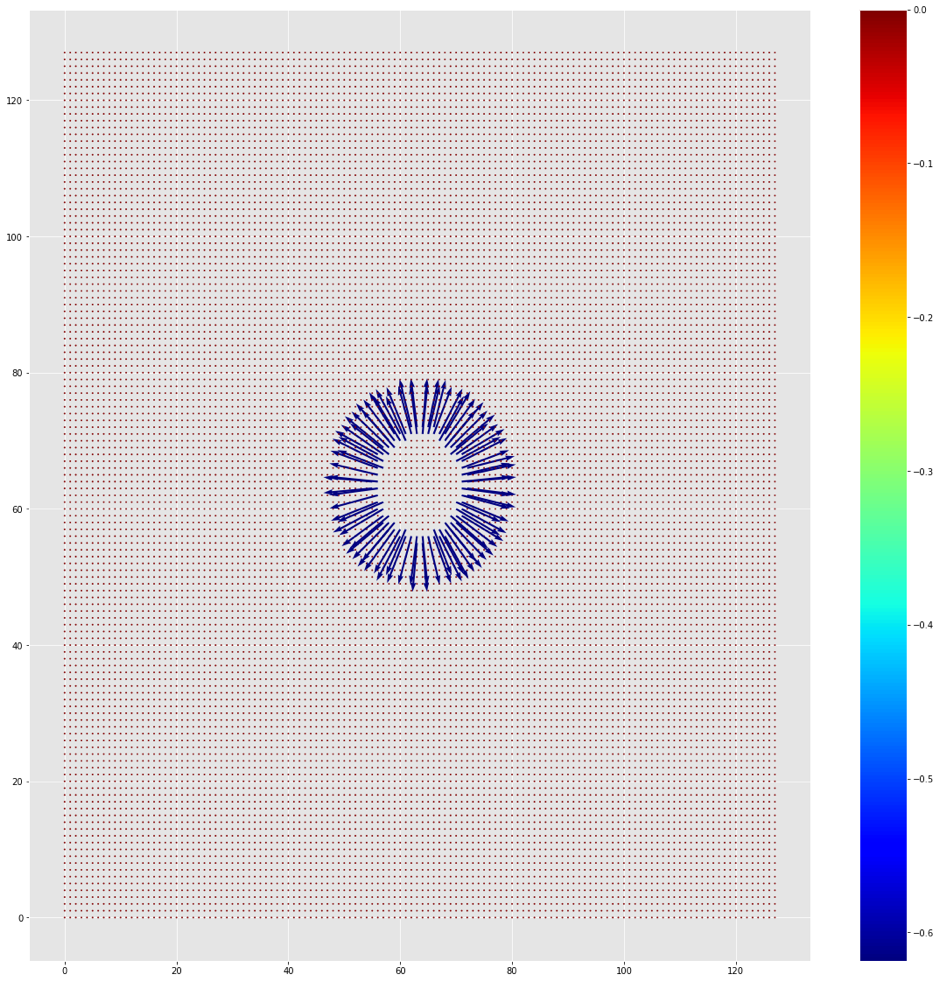
\includegraphics[width=0.9\textwidth]{Pictures/Level Set/level_set_velocity.png}
  \caption{Velocity visualized on a quiver plot}
  \label{img:microstrImg}
\end{subfigure}
\label{fig:test}
\end{figure}

% %%%%%%%%%%%%%%%%%%%%%%%%%%%%%%%%%%%%%%

\chapter{Hoshen-Kopelman Algorithm and Application}

\section{Formulation: General Hoshen-Kopelman}

The general Hoshen-Kopelman is one of the most efficient algorithms for cluster counting and labelling since it takes only one pass through the image to label the clusters in the image. We take a sample binary microstructure image and apply the regular Hoshen-Kopelman algorithm, which does not account for periodic boundary conditions to test our algorithm for Non-periodic images. The general algorithm without PBC is described as follows, without considering the boundary pixels:

\begin{algorithm}[H]
\SetAlgoLined
\KwResult{A matrix of labels}
 maxlabel=0\;
 \For{x in 0:no of columns and y in 0:n0 of rows}{

   \If{occupied[x,y]}{
   left = occupied[x-1,y]\;
   above = occupied[x,y-1]\;
    
    \If{left != 0 and above == 0}{
     label[x,y] = find(left)\;}
    \If{left == 0 and above != 0}{
     label[x,y] = find(above)\;}
    \If{left == 1 and above == 1}{
     union(left,above), \;
     label[x,y] = find(left)\;}
     
     }
   }
 \caption{Hoshen Kopleman algorithm for Non-PBC}
\end{algorithm}

Here, the union and find methods are derived from the common union-find algorithm. The union find algorithm is one of the most intensively studied and analyzed algorithms in the world, and I have implemented the \textbf{Weighted Union Find with Path Compression} technique to optimize the efficiency of the algorithm. The technique is useful as it can shorten the trees which are formed in the union find algorithms and also account for complexity in the nodes which are formed.

The Hoshen-Kopelman algorithm works well for non-periodic boundary conditions, but requires modifications for periodic boundary conditions. The specific problem with periodic boundary conditions is that the edge pixels could belong to the same cluster, and thus the above algorithm fails.

\section{Formulation : Hoshen Kopleman for PBC}
To account for periodic boundary conditions, we follow the original Hoshen-Kopelman algorithm to completion. Post completion, we run the algorithm again only on the edge labels/pixels with two key changes:

\begin{enumerate}
    \item We do not allot a new label value to a cluster encountered for the first time, instead we let it retain the earlier label
    \item We introduce the periodic boundary condition to the $1^{st}$ row and column of the image by defining it's left and above boundary pixel by adding a imaginary row and column to the left and top of the image. 
\end{enumerate}

The algorithm for periodic boundary conditions is as follows:

\begin{algorithm}[H]
\SetAlgoLined
\KwResult{A matrix of labels}
 maxlabel=0\;
 \For{x in 0:no of columns and y in 0:n0 of rows}{

  \If{occupied[x,y]}{
  left = occupied[x-1,y], \;
  above = occupied[x,y-1]\;
    
    \If{left != 0 and above == 0}{
     label[x,y] = find(left)\;}
    \If{left == 0 and above != 0}{
     label[x,y] = find(above)\;}
    \If{left == 1 and above == 1}{
     union(left,above), \;
     label[x,y] = find(left)\;}
    \If{left == 0 and above == 0}{
     maxlabel=maxlabel+1, \;
     label[x,y] = maxlabel\;}
     }
  }
  \For{x in 0:no of columns and y in 0:n0 of rows}{

  \If{occupied[x,y] and edge[x,y]}{
  left = occupied[x-1,y] considering periodicity, \;
  above = occupied[x,y-1] considering periodicity\;
    \If{left != 0 and above == 0}{
     label[x,y] = find(left)\;}
    \If{left == 0 and above != 0}{
     label[x,y] = find(above)\;}
    \If{left == 1 and above == 1}{
     union(left,above), \;
     label[x,y] = find(left)\;}
     }
  }
 \caption{Hoshen Kopleman algorithm for PBC}
\end{algorithm}

\section{Visualization}
We visualize the cluster labelled microstructure by color coding each precipitate based on its number. We can also visualize a single precipitate by projecting only one label.

\begin{figure}[H]
\centering
\begin{subfigure}{.6\textwidth}
  \centering
  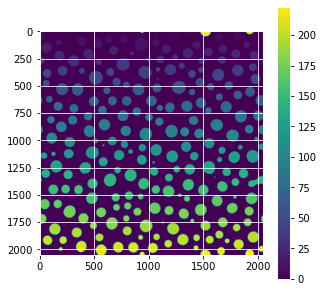
\includegraphics[width=0.9\textwidth]{Pictures/Hoshen/Hoshen_kopleman.jpeg}
  \caption{Cluster counting and labelling}
  \label{img:microstrImg}
\end{subfigure}
\label{fig:test}
\end{figure}


%%%%%%%%%%%%%%%%%%%%%%%%%%%%%%%%%%%%%%%%%%%%%%

\chapter{Shape/size quantification and Precipitate Tracking}

\section{Shape/size quantification}
Identifying features of precipitates like size, inclination etc can help us study precipitate growth and evolution in detail. Once we have identified a precipitate(by using the Hoshen-Kopelman algorithm), we can derive many features of the precipitate by analyzing the binary microstructure of the precipitate.

The two main proponents which are required to track and study a precipitate are the centre of gravity and the $2^{nd}$ order moment of the binary shape. The centre of gravity is associated with the spatial position of the precipitate and the moment is associated with the shape/inclination of the image. What makes it challenging is to extend the usually simplistic analysis on generic binary images to images with periodic boundary conditions. We will investigate the 2 problems separately in this section.

\subsection{Centre of gravity}
Centre of gravity for generic non-periodic binary images is directly obtained by orthogonal counting of precipitate pixels in both directions, and then finding the weighted mean of the resulting array. Since we are working with periodic boundary conditions, we first move from a linear array to an angular array, and do the weighted means in the rotational space. The physical equivalent of our approach would be folding the image to calculate the COG. The algorithm for one direction, say x, is described as follows. Given a directional array $x_i$ going from 1 to X and a weight distribution $m_i$ which adds up to $M$:

$\theta_i = \frac{2{\pi}x_i}{X}$

$\alpha_i = \cos{{\theta}_i}$
$\beta_i = \sin{{\theta}_i}$

$\Bar{\alpha_i} = \frac{1}{M}\sum_i {m_i}{\alpha_i} $          $\Bar{\beta_i} = \frac{1}{M}\sum_i {m_i}{\beta_i}$

$\Bar{\theta}$ $=$ arctan($-\Bar{\beta_i}$,$\Bar{\alpha_i}$)$+\pi$

\textbf{$X_{cog}$} =$\frac{X{\Bar{\theta}}}{2\pi}$

Thus we can find the Centre of gravity along the two orthogonal directions separately to get the final COG of a binary precipitate.

\subsection{Moments}
Once we have calculated the values of $X_{cog}$ and $Y_{cog}$, we can find the inclination, major and minor axis of a binary precipitate by using the values of second order moments. The $p^{th}$ and $q^{th}$ order moment of a binary image is calculated as follows:

$M_{pq} = \sum_{i,j{\in}Obj}i^pj^q$

We can thus calculate $M_{20}$, $M_{02}$, $M_{11}$ and $M_{00}$ from the above equation. We then calculate the following matrix and find the Eigen vectors and Eigen-values to get the inclination and major/minor axis.

$\mu_{20}$ = $\frac{M_{20}}{M_{00}}-{\Bar{x}}^2$
$\mu_{02}$ = $\frac{M_{02}}{M_{00}}-{\Bar{y}}^2$
$\mu_{11}$ = $\frac{M_{11}}{M_{00}}-{\Bar{x}}{\Bar{y}}$

$$
cov =
\begin{bmatrix}
\mu_{20} & \mu_{11} \\
\mu_{11} & \mu_{02} \\
\end{bmatrix}
$$

We can find the angle of inclination and major/minor axis by finding the eigen-vectors of the above matrix.


\section{Precipitate tracking}

Since our microstructures are evolving with time, it becomes imperative to track a particular precipitate and study it's growth. The Hoshen-Kopelman algorithm does an excellent job at counting the clusters and labelling them from 1 to n. The major problem faced in tracking is identifying which precipitate we are currently tracking, as the Hoshen-Kopelman labels will change for each precipitate in each time frame of image acquisition. That is, the Hoshen-Kopelman Algorithm can label the precipitates, but cannot tell us that 2 different labels corresponding to 2 different images across time are actually the same precipitate, which has grown/shrunk in the evolution process. 

The problem statement thus obtained is, given a \textbf{Hoshen-Kopelman Labelled Microstructure (HSLM)} image and the label of the precipitate being tracked, we need to find out the label for the same corresponding precipitate in the next/new \textbf{HSLM} image. We suggest 2 approaches to solve this problem:

\subsection{COG based tracking}
This approach relies on the fact that in gradually growing microstructure, the centre of gravity corresponding to a precipitate will lie on the same precipitate in the next time step of image acquisition. The flowchart below explains the steps in the algorithm.

\usetikzlibrary{shapes.geometric, arrows}
\tikzstyle{process} = [rectangle, minimum width=3cm, minimum height=1cm, text centered, draw=black]
\tikzstyle{arrow} = [thick,->,>=stealth]
\begin{center}
\begin{tikzpicture}[node distance=2cm]
\node (start) [process] {Binary Microstructure Image ($n^{th} image$)};
\node (in1) [process, below of=start] {Hoshen Kopleman Labelled Microstructure, Chosen Precipitate Label};
\node (in2) [process, below of=in1] {Centre of gravity of precipitate};
\node (in3) [process, below of=in2] {Label corresponding to COG in new HKLM (${(n+1)}^{th} image$)};
\node (in4) [process, below of=in3] {Precipitate in new microstructure (${(n+1)}^{th} image$)};
\draw [arrow] (start) -- (in1);
\draw [arrow] (in1) -- (in2);
\draw [arrow] (in2) -- (in3);
\draw [arrow] (in3) -- (in4);
\end{tikzpicture}
\end{center}

\subsection{Probabilistic tracking}
The primary issue with the COG based algorithms is the fact that as shape of precipitates move away from convexity, the Centre of Masses may or may not lie on the precipitate. Thus point based methods of tracking fail as the microstructure shapes grow more complex eg. Spinodal. Thus to solve this problem, we take a probabilistic approach of identifying the most likely precipitate in the ${(n+1)}^{th}$ image from the chosen precipitate in the $n^{th}$ image. Since we know that only a single precipitate in the ${(n+1)}^{th}$ image corresponds to the precipitate in the $n^{th}$ image, we simply superimpose the precipitate of study onto the ${(n+1)}^{th}$ image and find the cluster with the most number of pixels matching. That is, we identify which cluster of precipitates is most likely to be the precipitate we are studying.

This method can be formalized by the following process.
Given random variables representing coordinates $x,y\in{Image} $

Hoshen-Kopelman label for $n^{th}$ image: $(H_n) = f_n(x,y)$

Defining $P_n$ as the number associated with the precipitate being tracked from the HKLM.

In the above expression, $H_n = P_n \forall$ $x_n,y_n \in Precipitate$

We are required to find $P_{n+1}= H_{n+1}$, ie. the distribution of $x_{n+1},y_{n+1}$ such that the new distribution corresponds to the same precipitate. Formally :

$P_{n+1} = E(H_{n+1}| H_n = P_n ) = E(H_{n+1}|f_n(x_n,y_n)=P_n) = E(H_{n+1} | x_n,y_n \in Precipitate$)

The flowchart defines the steps taken:

\usetikzlibrary{shapes.geometric, arrows}
\tikzstyle{process} = [rectangle, minimum width=3cm, minimum height=1cm, text centered, draw=black]
\tikzstyle{arrow} = [thick,->,>=stealth]
\begin{center}
\begin{tikzpicture}[node distance=2cm]
\node (start) [process] {Binary Microstructure Image ($n^{th} image$)};
\node (in1) [process, below of=start] {Hoshen Kopleman Labelled Microstructure, Chosen Precipitate Label};
\node (in2) [process, below of=in1] {Binary mask previous precipitate on new HKLM(${(n+1)}^{th} image$)};
\node (in3) [process, below of=in2] {Label corresponding to most overlap in new HKLM (${(n+1)}^{th} image$)};
\node (in4) [process, below of=in3] {Precipitate in new microstructure (${(n+1)}^{th} image$)};
\draw [arrow] (start) -- (in1);
\draw [arrow] (in1) -- (in2);
\draw [arrow] (in2) -- (in3);
\draw [arrow] (in3) -- (in4);
\end{tikzpicture}
\end{center}



\section{Features/statistics investigation}

Once we have labelled the precipitate we are studying, we can calculate many quantitative parameters representing the precipitate distribution and shape/size. We list down parameters and features we can calculate:

\begin{enumerate}
    \item Centre of gravity and it's movement
    \item Precipitate size distribution
    \item Interface velocity
    \item Precipitate area change(growth/shrinking)
    \item Agglomeration of precipitates
    \item Sphericity and inclination
    \item Major and minor axis
    \item 2 point statistics of microstructure
    \item Convexity and concavity of precipitate
\end{enumerate}

\section{Flowchart describing process}

\usetikzlibrary{shapes.geometric, arrows}
\tikzstyle{process} = [rectangle, minimum width=3cm, minimum height=1cm, text centered, draw=black]
\tikzstyle{arrow} = [thick,->,>=stealth]
\begin{center}
\begin{tikzpicture}[node distance=2cm]
\node (start) [process] {Load microstructure images};
\node (in1) [process, below of=start] {Choose precipitate to track};
\node (in2) [process, below of=in1] {Track precipitate change as microstructure evolves};
\node (in3) [process, below of=in2] {At each time frame of acquisition, find relevant properties};
\node (in4) [process, below of=in3] {Plot property change to understand microstructure evolution};
\draw [arrow] (start) -- (in1);
\draw [arrow] (in1) -- (in2);
\draw [arrow] (in2) -- (in3);
\draw [arrow] (in3) -- (in4);
\end{tikzpicture}
\end{center}

\section{Visualization}
\begin{figure}[H]
\centering
\begin{subfigure}{.45\textwidth}
  \centering
  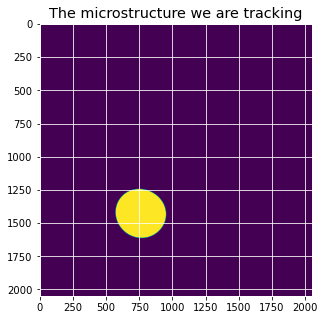
\includegraphics[width=0.9\textwidth]{Pictures/Tracking/Traching_cog.jpeg}
  \caption{COG suited precipitate}
  \label{img:microstrImg}
\end{subfigure}
\begin{subfigure}{.45\textwidth}
  \centering
  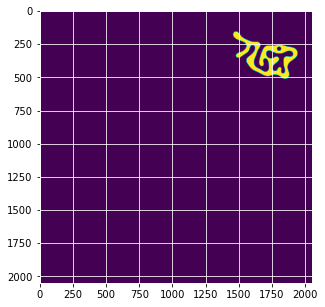
\includegraphics[width=0.9\textwidth]{Pictures/Tracking/Tracking_choosing_ppt.jpeg}
  \caption{Probabilistic model suited precipitate}
  \label{img:MicrostrImg}
\end{subfigure}
\caption{Visualizing Precipitates}
\label{fig:test}
\end{figure}

%%%%%%%%%%%%%%%%%%%%%%%%%%%%%%%%%%%%%%%%%%%
\chapter{Convexity measures}

\section{Definition}
We define Convexity in terms of a number called Convexity number, a probabilistic measure of how convex a binary image is. The convexity number should have the following features for it to be a good indicator of probability:
\begin{enumerate}
    \item A number lies between (0,1], with a perfectly convex shape having a value of 1
    \item The number increases as the convexity of the image increases
\end{enumerate}

A image is perfectly convex if given any 2 points taken on the image, the line joining the 2 points entirely lies in the image. Analogous to this definition, we define our convexity to measure the likeliness of this line joining 2 points on the image to lie on the image. The convexity measure we measure is the following:

\textit{Given 2 points on the image, what is the probability that a third point in the middle of these 2 points lies on the image as well.}

We simplify to account only for the midpoint since the midpoint lying on the line is often a good indicator of the whole line being on the line, and just calculating the midpoint saves us the computation time of calculating all the points in the line. The measure can thus be formally written as the following:


For points $p_i$ in the binary image space $I$ and $m_{ij}$ being the midpoints of 2 points $p_i$ and $p_j$ , we calculate:


$P_{convexity}$ = P($m_{ij} = 1$ $|$ $p_i = 1$ $\cap$ $p_j = 1$ )

This convexity measure is extremely difficult to compute, and theorems like the Convolution theorem we applied while calculating auto-correlations fail because of the presence of the extra midpoint term in the expression. We thus calculate this quantity by using Monte Carlo techniques.

% Add image of a concave and a convex precipitate here for understanding
\begin{figure}[H]
\centering
\begin{subfigure}{.45\textwidth}
  \centering
  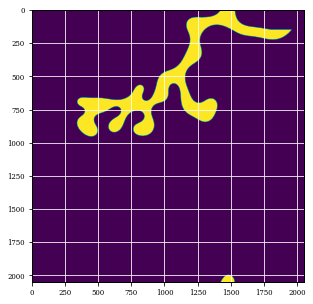
\includegraphics[width=0.9\textwidth]{Pictures/MSFeatures/ExampleConcavePPT.png}
  \label{img:microstrImg}
\end{subfigure}
\begin{subfigure}{.45\textwidth}
  \centering
  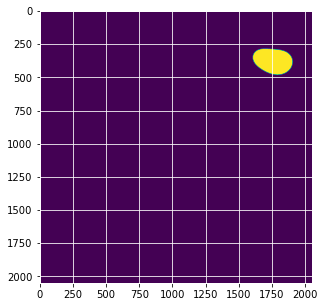
\includegraphics[width=0.9\textwidth]{Pictures/MSFeatures/ExampleConvexPPT.png}
  
  \label{img:microstrImg}
\end{subfigure}
\caption{Visualizing Concave and Convex shapes}
\label{fig:test}
\end{figure}



\section{Monte Carlo method}
Since calculating the exact probability measure is too computationally expensive, we use a Monte Carlo method to sample points from the image and calculate the probability measure. We run the simulation till the probability value converges, which we notice generally happens after 30,000 sampled points for 2000*2000 resolution images.

The formulation of the method is simple. We randomly select 2 points on the image which lie on the object. We then find the point in the middle of the line joining these 2 points, and check whether this point also lies in the object. The net probability measure we calculate then becomes:

$P_{convexity}$ = $\frac{\textit{No of midpoints on object}}{\textit{Number of pairs of points chosen on object}}$


\section{Testing convexity on precipitate growth}
We track 2 precipitates in the spinodal regime who can be observed to be moving towards convexity and test if our convexity measure in increasing in time and finally constant at 1 when the precipitate is perfectly convex. The 2 precipitates perfectly followed our hypothesis, which can be seen in the curves below. 

%% ADD 2 precipitate growth and increase curve
\begin{figure}[H]
\centering
\begin{subfigure}{.32\textwidth}
  \centering
  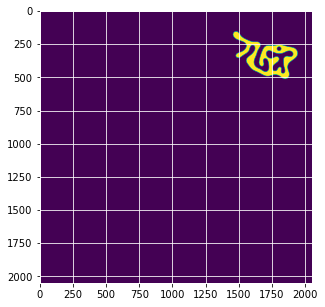
\includegraphics[width=0.9\textwidth]{Pictures/MSFeatures/ConvexMSStart.png}
  \label{img:microstrImg}
\end{subfigure}
\begin{subfigure}{.32\textwidth}
  \centering
  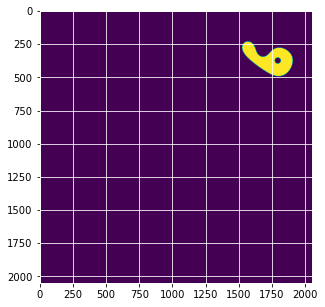
\includegraphics[width=0.9\textwidth]{Pictures/MSFeatures/ConvexMSMiddle.png}
  \label{img:microstrImg}
\end{subfigure}
\begin{subfigure}{.32\textwidth}
  \centering
  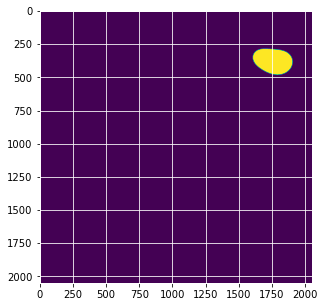
\includegraphics[width=0.9\textwidth]{Pictures/MSFeatures/ConvexMSEnd.png}
  \label{img:microstrImg}
\end{subfigure}
\begin{subfigure}{.5\textwidth}
  \centering
  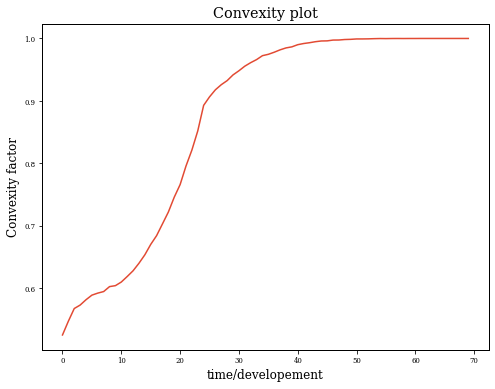
\includegraphics[width=0.9\textwidth]{Pictures/MSFeatures/IsoGrainConvexity.png}
  \label{img:microstrImg}
\end{subfigure}
\caption{Visualizing Convexity Number with Precipitate Growth}
\label{fig:test}
\end{figure}

\section{Convexity for complete microstructural images}
Since up until now we have talked only about convexity of individual precipitates, it only makes sense to define convexity in a form to quantify complete microstructural evolution with multiple precipitates. The traditional form of convexity that we define in the earlier section fails when we apply it to more than 1 precipitate in an image, and thus we require a new transformed form of convexity. 

We call this form of convexity \textbf{Short Range Averaged Convexity}. Rather than do the Monte Carlo random point sampling on the entire image, we break the image down into N$x$N smaller images, calculate the convexity for each of these smaller images(called Short Range Convexity), and report the average convexity of these smaller bits. This convexity can be imagined as a measure to ascertain at what length scale the microstructure is locally convex in. The flowchart describing the steps followed is as follows:

\usetikzlibrary{shapes.geometric, arrows}
\tikzstyle{process} = [rectangle, minimum width=3cm, minimum height=1cm, text centered, draw=black]
\tikzstyle{arrow} = [thick,->,>=stealth]
\begin{center}
\begin{tikzpicture}[node distance=2cm]
\node (start) [process] {Load microstructure image};
\node (in1) [process, below of=start] {Divide image into N*N tiles (eg. 4*4)};
\node (in2) [process, below of=in1] {Calculate the convexity of each tile(eg. 16 tiles)};
\node (in3) [process, below of=in2] {Report mean of convexity from all tiles};
\draw [arrow] (start) -- (in1);
\draw [arrow] (in1) -- (in2);
\draw [arrow] (in2) -- (in3);
\end{tikzpicture}
\end{center}

The Short Range Average Convexity values of a developing microstructure showed a steadily increasing value when using a N=4, ie. using 16 tiles. The microstructural evolution and the convexity values are shown below. We can see the steady increase in convexity values clearly with evolution, which verifies our model perfectly.

%% Add the images for micro growth and convexity short range
\begin{figure}[H]
\centering
\begin{subfigure}{.32\textwidth}
  \centering
  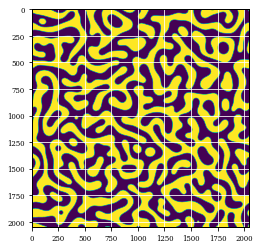
\includegraphics[width=0.9\textwidth]{Pictures/MSFeatures/ConvexMicroEvolStart.png}
  \label{img:microstrImg}
\end{subfigure}
\begin{subfigure}{.32\textwidth}
  \centering
  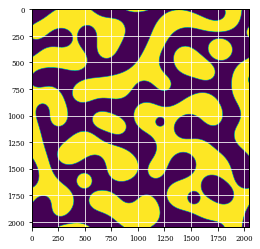
\includegraphics[width=0.9\textwidth]{Pictures/MSFeatures/ConvexMicroExalMiddle.png}
  \label{img:microstrImg}
\end{subfigure}
\begin{subfigure}{.32\textwidth}
  \centering
  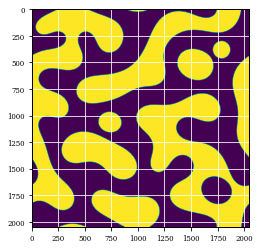
\includegraphics[width=0.9\textwidth]{Pictures/MSFeatures/ConvexMicroEvalEnd.png}
  \label{img:microstrImg}
\end{subfigure}
\begin{subfigure}{.5\textwidth}
  \centering
  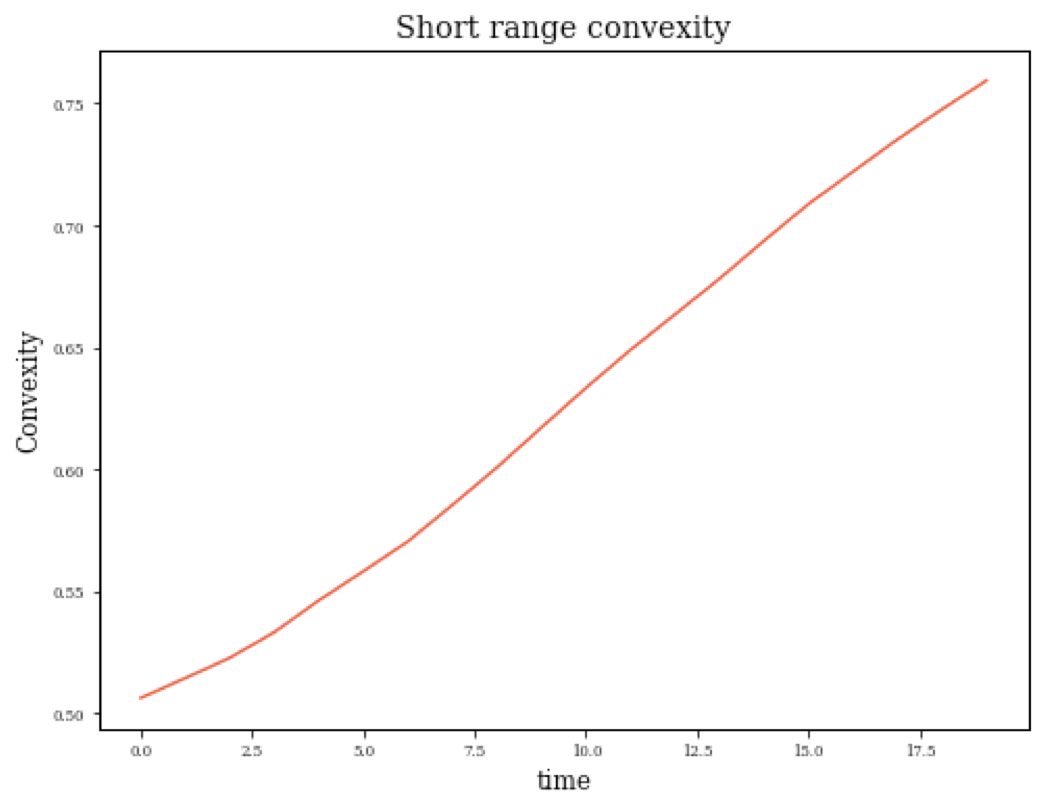
\includegraphics[width=0.9\textwidth]{Pictures/MSFeatures/ShortRangeConvexityIso.png}
  \label{img:microstrImg}
\end{subfigure}
\caption{Convexity number change with Microstructure Evolution}
\label{fig:test}
\end{figure}

%%%%%%%%%%%%%%%%%%%%%%%%%%%%%%%%%%%%%%%%%%%

\chapter{Results and Observations: Microstructure features}
In this section we compare the macroscopic properties of the Isotropic, Cubic and Hexagonal microstructures across time, and identify key distinguishing features between these properties. The macroscopic properties referred above relate to the Probabilistic Correlations of precipitates, precipitate count and distribution of precipitates in the generated periodic microstructures.

We use many of the techniques mentioned in the previous sections like the Hoshen-Kopelman algorithm and 2-point statistics to get these features. We compare between varying times/development of a single type of microstructure, and also between microstructure types (say Cubic and Hexagonal). This will give us a fair idea about the statistical parameters we can use to distinguish between these different types of microstructures, and can also play a key role in case we wish to interpolate and fit the time-series microstructures in a distribution.


\section{Datasets used for comparison}
The Cahn-Hilliard generated microstructures were of three types, the perfectly Isotropic, Hexagonal and Cubic. Each of these were generated for 200,000 time-steps, and every $200^{th}$ image was sampled out for analysis, ie. we had 1000 images to apply statistics to. Upon visual examination of these 1000 images, and noting down the statistical changes observed between different times , we observed that there was little significant change in statistical features between alternate images, ie. images 200 time-steps apart. Thus, to save on computing time we sample only every $30^{th}$  image out of the 100 images, which gives us enough time-series information to draw conclusions from, since within each 30 continuous images, the statistical difference is insignificant. 

In the next 2 sections (7.2 and 7.3), we explain the statistical parameters we calculate, and use the Hexagonal Microstructure as an example to demonstrate and visualize the parameters. In the later section (7.4), we compare these statistics across different types of microstructures (Isotropic, Hexagonal and Cubic).

\section{Correlations}
The 2-Point correlations are calculated as explained in Chapter 2. We visualize the precipitate cross-correlation and auto-correlation heat map, and also calculate these metrics on a distance scale, ie. calculating the values on a radial scale by averaging the probability along a thin circular ring. Furthermore, we extend this analysis to capture angular features along particular angular sectors, to capture anisotropy. Further details are mentioned in the succeeding sections.

\subsection{Auto-correlation and cross-correlations}
The auto-correlations represented as a probability heat-map is calculated for microstructures at different stages of their evolution. The points on the vector space(with the centre of the image as the origin) with color higher up on the color-bar represent higher probability of occurrence of the particular local state. For instance, at the centre(vector (0,0)), the probability will always be exactly equal to the probability of finding the local state(ie, 0.3 if we calculate auto-correlations for composition ~ 0.3). Furthermore, we can generally observe rings of higher and lower probability close to the origin, which are good indicators of the periodicity in the microstructures.  

For instance, in the below figures, you can observe the auto and cross correlations calculated for the isotropic case, which demonstrate the properties mentioned in the previous paragraph. We can clearly observe that the auto-correlations and cross-correlations for the isotropic microstructures have no directionality, and are perfectly spherically contoured as shown below. The high probability spherical rings are also perfectly visible around the centre, showing the approximate judgement of the precipitate sizes. 

% Add autocorr and cross corr for isotropic
\begin{figure}[H]
\centering
\begin{subfigure}{.32\textwidth}
  \centering
  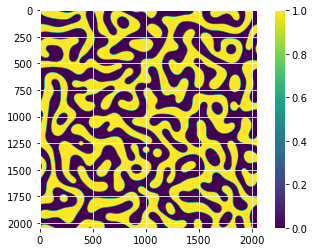
\includegraphics[width=0.9\textwidth]{Pictures/MSFeatures/CorrImageChosen.png}
  \label{img:microstrImg}
\end{subfigure}
\begin{subfigure}{.32\textwidth}
  \centering
  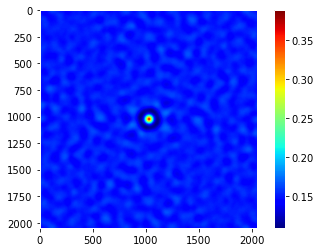
\includegraphics[width=0.9\textwidth]{Pictures/MSFeatures/CorrImageAuto.png}
  \label{img:microstrImg}
\end{subfigure}
\begin{subfigure}{.32\textwidth}
  \centering
  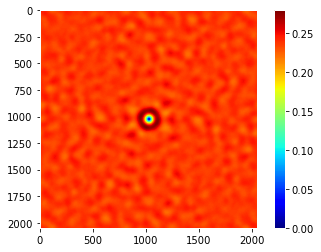
\includegraphics[width=0.9\textwidth]{Pictures/MSFeatures/CorrImageCross.png}
  \label{img:microstrImg}
\end{subfigure}
\caption{Visualizing Correlation for Isotropic Microstructures}
\label{fig:test}
\end{figure}

For the hexagonal microstructure, visualizing the probability correlation heatmap gives expected results. For the hexagonal case, we can clearly see the anisotropy in the precipitate distribution in the figures below in the form of the hexagons of high and low probability around the centre, which adds credence to our formulation. 

% Add autocorr and cross corr for hexa
\begin{figure}[H]
\centering
\begin{subfigure}{.32\textwidth}
  \centering
  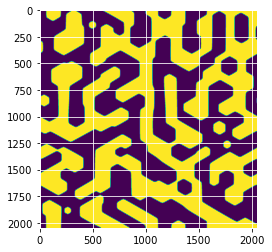
\includegraphics[width=0.9\textwidth]{Pictures/MSFeatures/CorrHexaImage.png}
  \label{img:microstrImg}
\end{subfigure}
\begin{subfigure}{.32\textwidth}
  \centering
  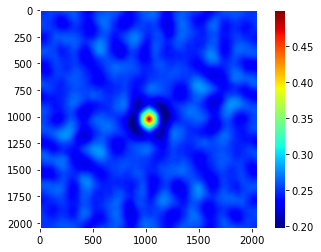
\includegraphics[width=0.9\textwidth]{Pictures/MSFeatures/CorrHexaAuto.png}
  \label{img:microstrImg}
\end{subfigure}
\begin{subfigure}{.32\textwidth}
  \centering
  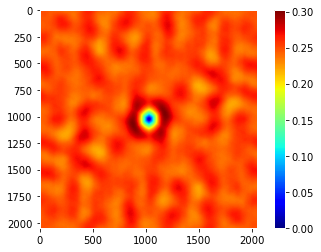
\includegraphics[width=0.9\textwidth]{Pictures/MSFeatures/CorrHexaCross.png}
  \label{img:microstrImg}
\end{subfigure}
\caption{Visualizing Correlation for Hexagonal Microstructures}
\label{fig:test}
\end{figure}
By using these Correlation heatmaps, we can get a fair idea about the anisotropy shape/directions, and also judge the particle sizes by looking at the sized of the rings around the centre. Thus, these heatmaps capture important macroscopic features from the binary microstructure images. 


\subsection{Radial Auto-correlation and Cross-correlation}

Although the correlation heatmaps give us significant information about the anisotropy and approximate sizes of the precipitates, these are not numerically quantifiable and easily visualized through only the heatmaps. Thus we plot the radial correlations as a measure, derived directly from the probability heatmaps above, which can quantify the understanding of the particle sizes. 

We define the radial auto-correlation as the auto-correlation taken and averaged at a particular radial distance. This is calculated by simply taking a correlation plot, and finding the average probability at thin rings of radius $r$ around the centre. This way, we can capture more easily the particle distribution at a radial distance $r$ from the origin. This plot gives us important information about the probability distribution of precipitates, and can help us identify the particle size and inter particle distance of a microstructure. 

The x coordinate represents the radial distance from the origin, while the y axis represents the probability of finding the same local state(in our auto-correlations case - the precipitate) at that radial distance. The first x-coordinate minima of the radial auto-correlation curve corresponds to the particle size(ie. where the likelyhood of finding the precipitate is lowest), while the first maxima after the origin is an indication of the inter-particle distance(ie. where the likelyhood of finding another precipitate is highest again).

These 2 measures can be plotted across time to study particle size growth and distribution in microstructural evolution. As we can observe in the figures below for the Hexagonal Microstructures as an example, the plots are largely oscillatory, implying subsequent higher and lower probability regions of precipitate in a microstructure, which holds well with our microstructural image. Furthermore, as we make this plot at increasing intervals of time, the curve moves towards the rights, ie. the precipitate size and inter-particle distance both increase as the microstructure develops, which also holds true with our images.

Most importantly, the difference in probability values of precipitates at difference compositions in the figure below clearly shows us how composition changes affect particle sizes and distances.

% Add image for radial autocorr and crosscorr one each
\begin{figure}[H]
\centering
\begin{subfigure}{.9\textwidth}
  \centering
  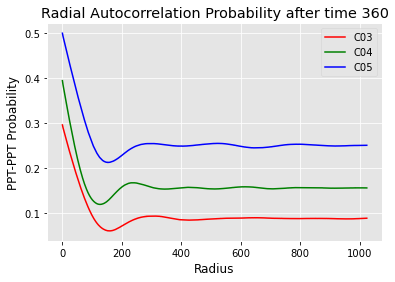
\includegraphics[width=0.9\textwidth]{Pictures/MSFeatures/RadialCorrExample.png}
  \label{img:microstrImg}
\end{subfigure}
\caption{Plotting Radial Auto Correlations}
\label{fig:test}
\end{figure}

%radial change with time plotted
\begin{figure}[H]
\centering
\begin{subfigure}{.48\textwidth}
  \centering
  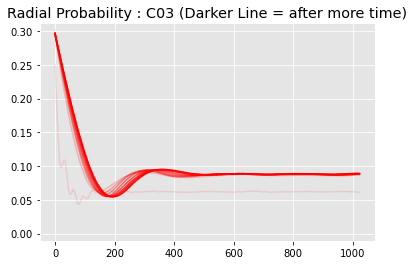
\includegraphics[width=0.95\textwidth]{Pictures/MSFeatures/RadialCorrTime1.png}
  \label{img:microstrImg}
\end{subfigure}
\begin{subfigure}{.48\textwidth}
  \centering
  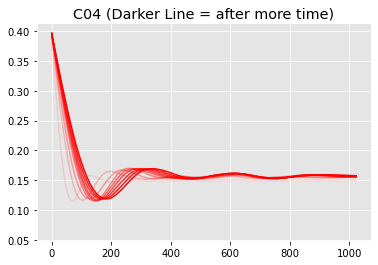
\includegraphics[width=0.95\textwidth]{Pictures/MSFeatures/radialCorrTime2.png}
  \label{img:microstrImg}
\end{subfigure}
\begin{subfigure}{.48\textwidth}
  \centering
  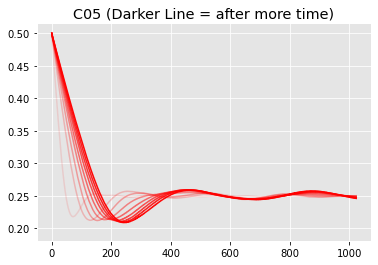
\includegraphics[width=0.95\textwidth]{Pictures/MSFeatures/RadialCorrTime3.png}
  \label{img:microstrImg}
\end{subfigure}

\caption{Plotting radial auto-correlations vs time}
\label{fig:unexplainablePlot}
\end{figure}

The radial auto-correlation change with time gives us a good indication of precipitate growth as the we can clearly see the radial curve spread out/decrease in frequency as the microstructure evolves.

\textbf{An interesting observation here is that the x-coordinate minima or the average particle size of concentration 0.3 and 0.4 are almost identical, ie. larger precipitates are not seen at a higher composition of 0.4.}

\subsection{Angular Auto correlations}
In cases of anisotropy, it becomes imperative to establish precipitate growth in different directions, as a single radial correlation does not give us information about the anisotropy in the system. This can be done simply by plotting the radial correlation only between certain angles ie. sectors to compare the evolution along these angles. That is, rather than calculating the mean probability over a ring around the origin, we calculate the mean along an angular arc on the ring. 

This can be done in 2 ways, comparing growth/size along a particular direction to the average growth/size, and identifying directions of anisotropy. This itself becomes a test for anisotropy, as a perfectly isotropic microstructure will show identical radial behavior along all angles and directions.

% Plot of radial vs 3060 degree
\begin{figure}[H]
\centering
\begin{subfigure}{.49\textwidth}
  \centering
  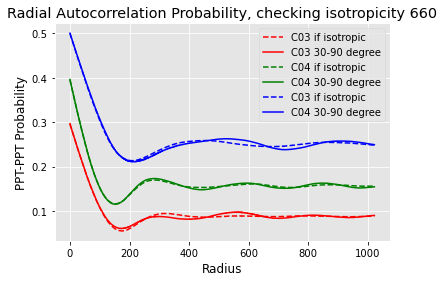
\includegraphics[width=0.95\textwidth]{Pictures/MSFeatures/ShowingAnisotropyAngle.png}
  \label{img:microstrImg}
  \caption{Comparing radial and angular correlation as an anisotropy test}
\end{subfigure}
\begin{subfigure}{.49\textwidth}
  \centering
  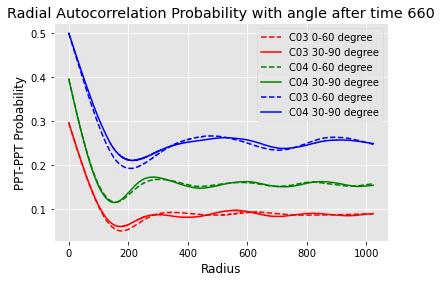
\includegraphics[width=0.95\textwidth]{Pictures/MSFeatures/RadialCorr306090Comparison.png}
  \caption{Comparing 2 different angles of growth}
  \label{img:microstrImg}
\end{subfigure}

\caption{Comparing directional growth}
\label{fig:test}
\end{figure}

We can also compare angles of growth to understand in which directions the anisotropy is prominent. We compare 2 sectors of 60 degrees in the curves above.

\section{Precipitate Counting and distribution Statistics}

\begin{figure}[H]
\centering
\begin{subfigure}{.45\textwidth}
  \centering
  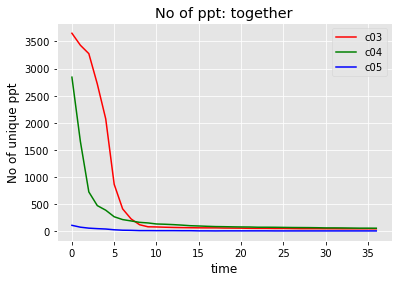
\includegraphics[width=0.9\textwidth]{Pictures/PPTCount/ParticleSizeDist.png}
  \caption{Plotting number of particles}
  \label{img:microstrImg}
\end{subfigure}
\begin{subfigure}{.45\textwidth}
  \centering
  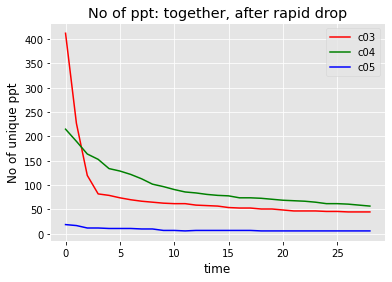
\includegraphics[width=0.9\textwidth]{Pictures/PPTCount/ParticleSizeDistAfterDrop.png}
  \caption{Close up view of particle count}
  \label{img:microstrImg}
\end{subfigure}
\caption{Particle Counting with time}
\label{fig:test22}
\end{figure}
Since we have implemented the Hoshen-Kopelman algorithms to segment individual clusters of precipitates, we can also easily capture the macroscopic properties like the number of precipitates, average precipitate size, standard deviation etc across both composition and time. These features are more prominently versatile in the initial time periods of microstructural development, and asymptotically converge as the microstructure grows to larger precipitates. 

For instance, the figure below shows the mean, standard deviation and precipitate count comparison of Hexagonal microstructures across time. 

\begin{figure}[H]
\centering
\begin{subfigure}{.45\textwidth}
  \centering
  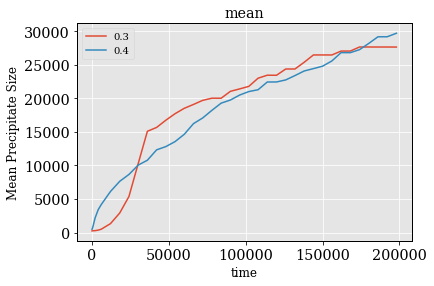
\includegraphics[width=0.9\textwidth]{Pictures/MSFeatures/mean_size.png}
  \caption{Mean}
  \label{img:microstrImg}
\end{subfigure}
\begin{subfigure}{.45\textwidth}
  \centering
  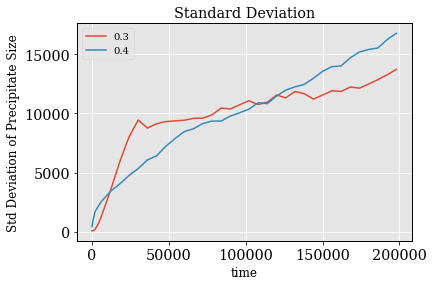
\includegraphics[width=0.9\textwidth]{Pictures/MSFeatures/std_size.png}
  \caption{Std. Deviation}
  \label{img:microstrImg}
\end{subfigure}
\begin{subfigure}{.45\textwidth}
  \centering
  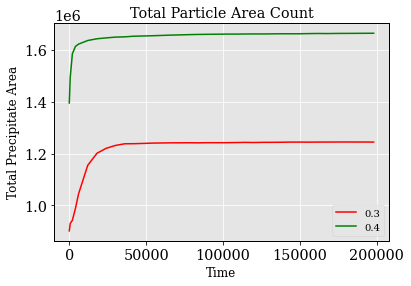
\includegraphics[width=0.9\textwidth]{Pictures/MSFeatures/total_size.png}
  \caption{Total Precipitate Area}
  \label{img:microstrImg}
\end{subfigure}
\caption{Precipitate Size statistics}
\label{fig:test22}
\end{figure}

Furthermore, we can also try and fit the precipitate areas into a area and log area distribution to better understand the precipitate size distribution by plotting histograms. The histograms are only useful with large number of precipitates in the image, and are usually useful only within the initial stages of the microstructure development. The typical histograms of really early stage microstructures like like the figure below.

\begin{figure}[H]
\centering
\begin{subfigure}{.9\textwidth}
  \centering
  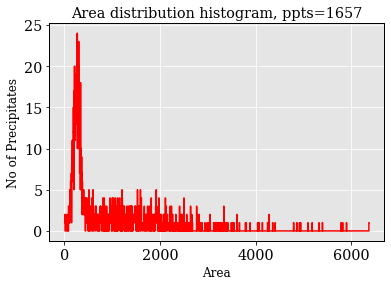
\includegraphics[width=0.9\textwidth]{Pictures/MSFeatures/Area_hist.png}
  \caption{Precipitate Size Distribution}
  \label{img:microstrImg}
\end{subfigure}
\label{fig:test22}
\end{figure}

% What is interesting to note here is that when we compare the microstructural evolution of composition 0.3 and 0.4, the particle size remains almost the same in both cases, which sounds non-intuitive since C0.4 has a greater concentration of the component controlling precipitate formation. The first curve shows that as the microstructure evolves, the number of precipitates reduce, which shows that growth has taken place and smaller precipitates have either vanished or agglomerated with the bigger precipitates. The second figure, which is a zoomed-in image of the first plot (to the right end of the time series data), shows that the number of precipitates in the 0.4 composition are more than the ones at 0.3. This means that even though the average precipitate size remains almost identical in 0.4 to 0.3, the number of precipitates with that size have increased. This means that when we go from C0.3 to C0.4, the additional composition is used in forming more precipitates rather than growing the present precipitates to larger sizes. This explains the ambiguity we saw in Section 7.2 and Fig. \ref{fig:unexplainablePlot}.

\section{Comparison between Isotropic, Hexagonal and Cubic}
\subsection{Auto-Correlation Heat-maps}


\subsection{Radial Correlations}


\subsection{Precipitate Size Statistics}

%%%%%%%%%%%%%%%%%%%%%%%%%%%%%%%%%%%%%%%%%%%
%%%%%%%%%%%%%%%%%%%%%%%%%%%%%%%%%%%%%%%%%%%
\chapter{Results and Observations: Precipitate tracking}

\section{C=0.3}
We consider a microstructure growth with a composition of 0.3 for the minor component and study 2 special grain growth cases.

\subsection{Directional growth}
Some precipitates grow more in a particular direction non-uniformly, due to the presence of external precipitate distributions. Up until now, to detect whether a precipitate is growing non-uniformly was a manual process. We suggest a technique where we run our algorithm on the chosen precipitate and track it's growth, and identify whether the COG of the precipitate is moving from position. 

\begin{figure}[H]
\centering
\begin{subfigure}{.24\textwidth}
  \centering
  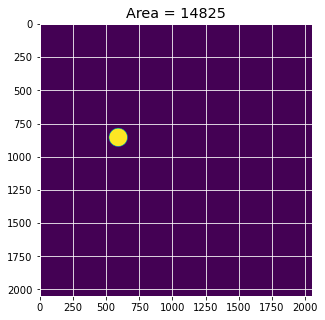
\includegraphics[width=0.9\textwidth]{Pictures/Growth/1.1.jpeg}
  \label{img:microstrImg}
\end{subfigure}
\begin{subfigure}{.24\textwidth}
  \centering
  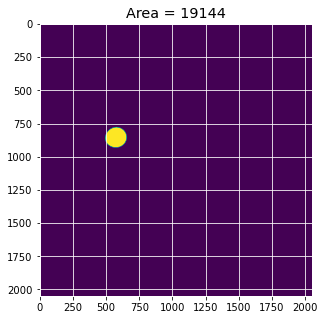
\includegraphics[width=0.9\textwidth]{Pictures/Growth/1.2.jpeg}
  \label{img:microstrImg}
\end{subfigure}
\begin{subfigure}{.24\textwidth}
  \centering
  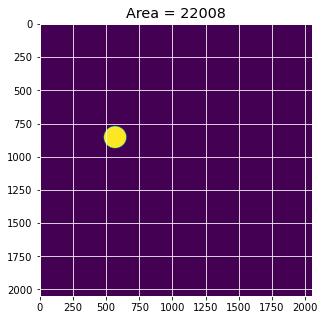
\includegraphics[width=0.9\textwidth]{Pictures/Growth/1.3.jpeg}
  \label{img:microstrImg}
\end{subfigure}
\begin{subfigure}{.24\textwidth}
  \centering
  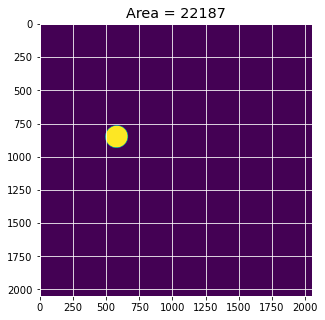
\includegraphics[width=0.9\textwidth]{Pictures/Growth/1.4.jpeg}
  \label{img:microstrImg}
\end{subfigure}
\label{fig:test}
\end{figure}

In bi-directional symmetric growth, although the axis of the precipitate might grow, the COG remains largely steady. The movement of the COG in a particular direction is a indication of how uni-directional the precipitate growth is. The figure below illustrates the phenomenon.

\begin{figure}[H]
\centering
\begin{subfigure}{.45\textwidth}
  \centering
  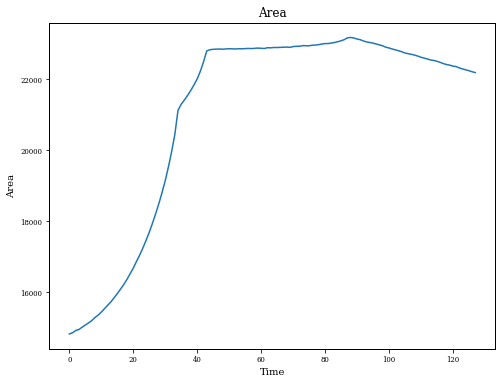
\includegraphics[width=0.9\textwidth]{Pictures/Results/1area.jpeg}
  \caption{Area/precipitate growth}
  \label{img:microstrImg}
\end{subfigure}
\begin{subfigure}{.45\textwidth}
  \centering
  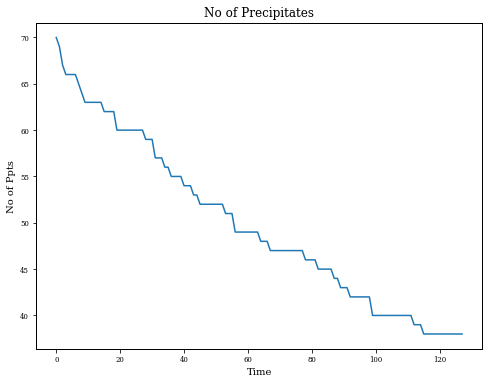
\includegraphics[width=0.9\textwidth]{Pictures/Results/1ppts.jpeg}
  \caption{Precipitate count}
  \label{img:microstrImg}
\end{subfigure}
\begin{subfigure}{.45\textwidth}
  \centering
  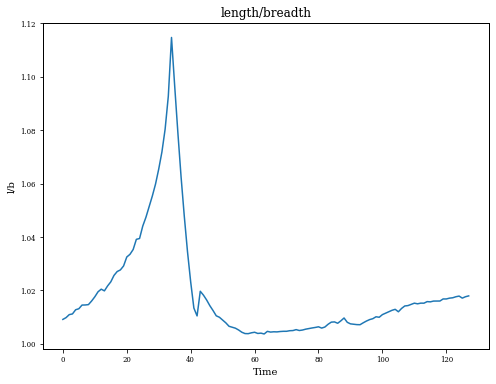
\includegraphics[width=0.9\textwidth]{Pictures/Results/1lb.jpeg}
  \caption{Studying sphericity}
  \label{img:microstrImg}
\end{subfigure}
\begin{subfigure}{.45\textwidth}
  \centering
  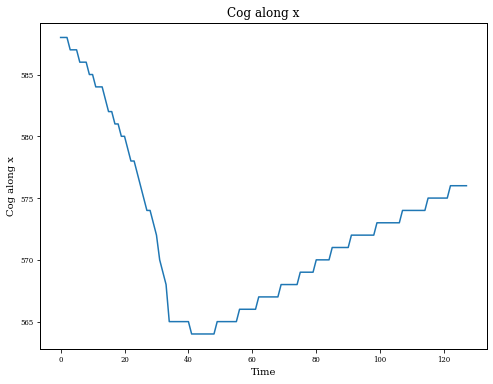
\includegraphics[width=0.9\textwidth]{Pictures/Results/1cogx.jpeg}
  \caption{The x coordinate of COG shows a trough, indicating left sided growth}
  \label{img:microstrImg}
\end{subfigure}
\caption{Precipitate parameter visualization}
\label{fig:test}
\end{figure}

\subsection{Identifying agglomeration}
Many times, 2 precipitates agglomerate to form a single precipitate. Identification of such types of agglomeration is easily notices by observing the discontinuities in the area of the tracked precipitate. The point of agglomeration sees a significant jump in the precipitate tracked area. Furthermore the sphericity ($\frac{l}{b}$) also sees a jump, since agglomeration starts with an elongated structure.
\begin{figure}[H]
\centering
\begin{subfigure}{.24\textwidth}
  \centering
  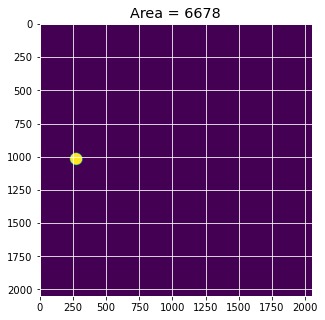
\includegraphics[width=0.9\textwidth]{Pictures/Growth/2.1.jpeg}
  \label{img:microstrImg}
\end{subfigure}
\begin{subfigure}{.24\textwidth}
  \centering
  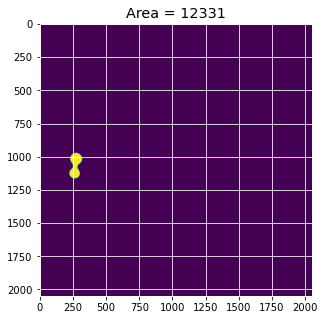
\includegraphics[width=0.9\textwidth]{Pictures/Growth/2.2.jpeg}
  \label{img:microstrImg}
\end{subfigure}
\begin{subfigure}{.24\textwidth}
  \centering
  \includegraphics[width=0.9\textwidth]{Pictures/Growth/2.3.jpeg}
  \label{img:microstrImg}
\end{subfigure}
\begin{subfigure}{.24\textwidth}
  \centering
  \includegraphics[width=0.9\textwidth]{Pictures/Growth/2.4.jpeg}
  \label{img:microstrImg}
\end{subfigure}
\label{fig:test}
\end{figure}

\begin{figure}[H]
\centering
\begin{subfigure}{.45\textwidth}
  \centering
  \includegraphics[width=0.9\textwidth]{Pictures/Results/2area.jpeg}
  \caption{Discontinuity in area implies start of agglomeration}
  \label{img:microstrImg}
\end{subfigure}
\begin{subfigure}{.45\textwidth}
  \centering
  \includegraphics[width=0.9\textwidth]{Pictures/Results/2lb.png}
  \caption{Sudden elongation is presage to future agglomeration}
  \label{img:microstrImg}
\end{subfigure}
\begin{subfigure}{.45\textwidth}
  \centering
  \includegraphics[width=0.9\textwidth]{Pictures/Results/2angle.jpeg}
  \caption{Angle of inclination determines direction of agglomeration}
  \label{img:microstrImg}
\end{subfigure}
\caption{Agglomeration: We go to the time where area becomes discontinuous, and continue tracking henceforth}
\label{fig:test}
\end{figure}

\section{C=0.4}

\subsection{Precipitate inclination}
The presence of a perfectly spherical precipitate leads to no angle of inclination, so in such cases random noise is observed. But most often, due to anisotropy, we generally observe a detectable angle of inclination. We study one such precipitate growth here, where the inclination is easily observable.

\begin{figure}[H]
\centering
\begin{subfigure}{.24\textwidth}
  \centering
  \includegraphics[width=0.9\textwidth]{Pictures/Growth/3.1.jpeg}
  \label{img:microstrImg}
\end{subfigure}
\begin{subfigure}{.24\textwidth}
  \centering
  \includegraphics[width=0.9\textwidth]{Pictures/Growth/3.2.jpeg}
  \label{img:microstrImg}
\end{subfigure}
\begin{subfigure}{.24\textwidth}
  \centering
  \includegraphics[width=0.9\textwidth]{Pictures/Growth/3.3.jpeg}
  \label{img:microstrImg}
\end{subfigure}
\begin{subfigure}{.24\textwidth}
  \centering
  \includegraphics[width=0.9\textwidth]{Pictures/Growth/3.4.jpeg}
  \label{img:microstrImg}
\end{subfigure}
\label{fig:test}
\end{figure}

\begin{figure}[H]
\centering
\begin{subfigure}{.45\textwidth}
  \centering
  \includegraphics[width=0.9\textwidth]{Pictures/Results/3area.jpeg}
  \caption{We observe a steady precipitate growth}
  \label{img:microstrImg}
\end{subfigure}
\begin{subfigure}{.45\textwidth}
  \centering
  \includegraphics[width=0.9\textwidth]{Pictures/Results/3lb.jpeg}
  \caption{The elongation is easily observable}
  \label{img:microstrImg}
\end{subfigure}
\begin{subfigure}{.45\textwidth}
  \centering
  \includegraphics[width=0.9\textwidth]{Pictures/Results/3theta.jpeg}
  \caption{The angle hovers around the $\frac{\pi}{6}$ mark}
  \label{img:microstrImg}
\end{subfigure}
\caption{Inclination is easily observable in the tracked precipitates}
\label{fig:test}
\end{figure}

\section{C=0.5}
\subsection{Moving towards convexity}
While tackling really complex shapes, we prefer to use the probabilistic method of tracking the precipitate, which is uniquely able to track precipitates with really non-convex shapes. 

\begin{figure}[H]
\centering
\begin{subfigure}{.24\textwidth}
  \centering
  \includegraphics[width=0.9\textwidth]{Pictures/Growth/4.1.jpeg}
  \label{img:microstrImg}
\end{subfigure}
\begin{subfigure}{.24\textwidth}
  \centering
  \includegraphics[width=0.9\textwidth]{Pictures/Growth/4.2.jpeg}
  \label{img:microstrImg}
\end{subfigure}
\begin{subfigure}{.24\textwidth}
  \centering
  \includegraphics[width=0.9\textwidth]{Pictures/Growth/4.3.jpeg}
  \label{img:microstrImg}
\end{subfigure}
\begin{subfigure}{.24\textwidth}
  \centering
  \includegraphics[width=0.9\textwidth]{Pictures/Growth/4.4.jpeg}
  \label{img:microstrImg}
\end{subfigure}
\begin{subfigure}{.24\textwidth}
  \centering
  \includegraphics[width=0.9\textwidth]{Pictures/Growth/4.5.jpeg}
  \label{img:microstrImg}
\end{subfigure}
\label{fig:test}
\end{figure}

\begin{figure}[H]
\centering
\begin{subfigure}{.45\textwidth}
  \centering
  \includegraphics[width=0.9\textwidth]{Pictures/Results/4area.jpeg}
  \caption{We observe a steady precipitate growth}
  \label{img:microstrImg}
\end{subfigure}
\begin{subfigure}{.45\textwidth}
  \centering
  \includegraphics[width=0.9\textwidth]{Pictures/Results/4lb.jpeg}
  \caption{The elongation is easily observable}
  \label{img:microstrImg}
\end{subfigure}
\caption{Such complex shaped precipitates can be tracked by using Probabilistic models as usual methods fail.}
\label{fig:test}
\end{figure}

Note: An important observation in such concave microstructures is the inherent movement towards convexity, which we have dealt with in previous precipitates.

%%%%%%%%%%%%%%%%%%%%%%%%%%%%%%%%%%%%%%%%%%%%%%
%%%%%%%%%%%%%%%%%%%%%%%%%%%%%%%%%%%%%%%%%%%%%%







\end{document}          
